\documentclass[12pt]{article}
\usepackage{graphicx}
\begin{document}
\title{Lista 2 - Piramide Usando OpenGL - SDL2}
\author{Mac\'artur de Sousa Carvalho}
\maketitle

\section{Solu\c{c}\~ao Proposta}
	Neste exercicio foi gerado um implementa\c{c}\~ao para renderiza\c{c}\~ao de uma piramide utilizando a biblioteca SDL e OPENGL para criar uma piramide apartir de informa\c{c}\~oes de um arquivo.Ao executar esta solu\c{c}\~ao utilizando pontos de um arquivo txt dispostos como exposto \'e possivel gerar uma piramide utilizando linhas e tamb\'em utilizando-se colunas.

\section{Caracter\'isticas da Solu\c{c}\~ao}
	Est\'a solu\c{c}\~ao consta de um programa capas de capturar entradas de um arquivo e renderizar uma piramide aparter dos pontos passados, na qual sempre deve-se descrever a quantidade de pontos que ser\'a utilizado e ent\~a determinar quais os pontos que ser\~ao utilizados para formar as arestas ou os poligonos da figura.

\section{Principais Li\c{c}\~oes Aprendidas}
	Com este exercicio foi possivel entender melhor o funcionamento do opengl ao desenhar uma figura geom\'etrica , isso ajuda muita no momento de criar um programa que possua varios poligonos.

\section{Principais Dificuldades Encontradas}
	Uma das grandes dificuldades encontradas na cria\c{c}\~ao de um programa que mostre um objeto em 3d \'e posicionalo na tela para uma melhor visualiza\c{c}\~ao do usu\'ario, muitas fezes não \'e poss\'ivel visualizar o que est\'a ocorrendo de errado com a renderiza\c{c}\~ao na tela , no entando  muitas vezes o motivo da não visualiza\c{c}\~ao é os pontos colocados em lugares que n\~ao s\~ao visualizados.


\section{Imagem solu\c{c}\~ao proposta}

\begin{figure}[!htb]
\centering
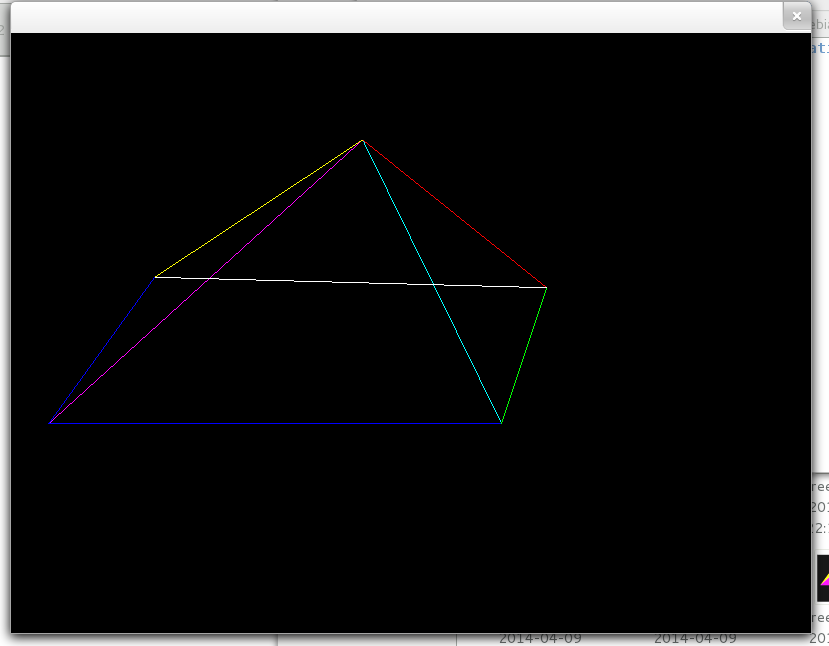
\includegraphics[scale=0.5]{images/piramide_linha.png}
\caption{Figura utilizando Linhas(Vertices) de uma piramide}
\end{figure}

\begin{figure}[!htb]
\centering
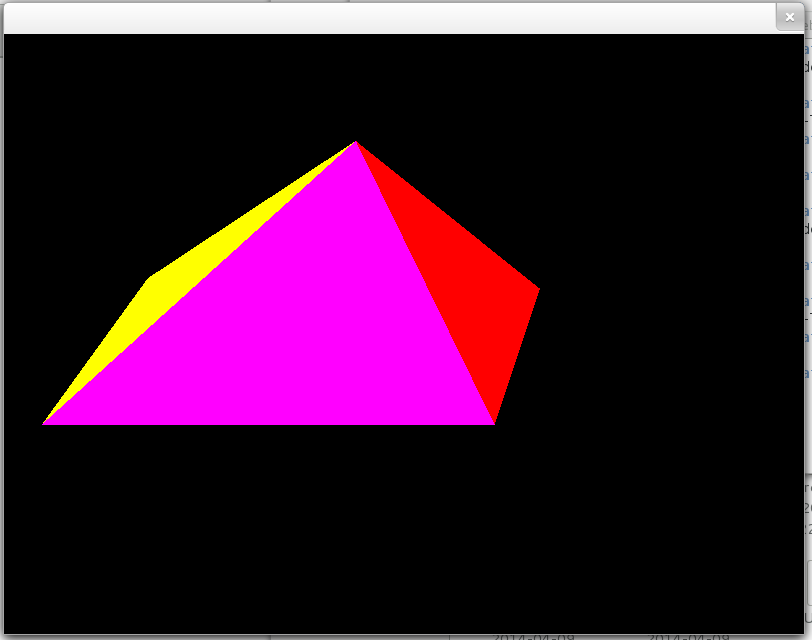
\includegraphics[scale=0.5]{images/piramide_poligono.png}
\caption{Figura utilizando poligonos para formar uma piramide}
\end{figure}

\end{document}




